\documentclass[tikz,border=6pt]{standalone}
\usepackage[T1]{fontenc}
\usepackage{helvet}
\renewcommand{\familydefault}{\sfdefault}
\usetikzlibrary{arrows.meta}
\tikzset{
  box/.style={draw,thick,minimum width=2.8cm,minimum height=1.1cm,align=center,font=\small},
  arr/.style={-{Stealth[length=2.5mm]},thick},
  lbl/.style={font=\bfseries\small,anchor=west}
}
\begin{document}
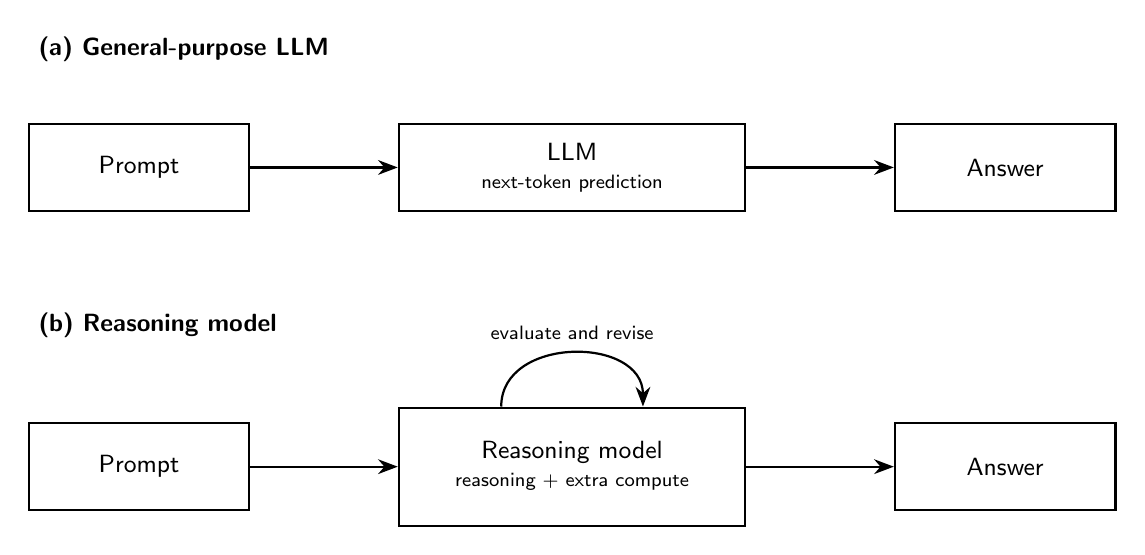
\begin{tikzpicture}
  % (a) General-purpose LLM
  \node[lbl] at (0,1.5) {(a) General-purpose LLM};
  \node[box] (p1) at (1.4,0) {Prompt};
  \node[box,minimum width=4.4cm] (l) at (6.9,0)
    {LLM\\[-1pt]{\scriptsize next-token prediction}};
  \node[box] (o1) at (12.4,0) {Answer};
  \draw[arr] (p1) -- (l);
  \draw[arr] (l) -- (o1);

  % (b) Reasoning model
  \node[lbl] at (0,-2.0) {(b) Reasoning model};
  \node[box] (p2) at (1.4,-3.8) {Prompt};
  \node[box,minimum width=4.4cm,minimum height=1.5cm] (r) at (6.9,-3.8)
    {\begin{tabular}{c}
      Reasoning model\\[-1pt]
      {\scriptsize reasoning + extra compute}
    \end{tabular}};
  \node[box] (o2) at (12.4,-3.8) {Answer};
  \draw[arr] (p2) -- (r);
  \draw[arr] (r) -- (o2);
  \draw[arr] ([xshift=-0.9cm]r.north) .. controls +(0,0.9) and +(0,0.9) .. ([xshift=0.9cm]r.north);
  \node[font=\scriptsize] at (6.9,-2.1) {evaluate and revise};
\end{tikzpicture}
\end{document}
